\renewcommand{\thesubsection}{\textcolor{red}{\Roman{section}.\arabic{subsection}}}
\renewcommand{\thesubsubsection}{\textcolor{red}{\Roman{section}.\arabic{subsection}.\alph{subsubsection}}}

\setcounter{section}{0}
\sndEnTeteExerciceDeux

\begin{center}
\begin{mdframed}[style=titr, leftmargin=60pt, rightmargin=60pt, innertopmargin=7pt, innerbottommargin=7pt, innerrightmargin=8pt, innerleftmargin=8pt]

\begin{center}
\large{\textbf{Feuille d'exercices du Chapitre 2}}
\end{center}

\end{mdframed}
\end{center}

\section{Pour commencer}
\begin{mdframed}[style=autreexo]
\textbf{\bsc{Exercice 1} - Entoure la bonne réponse} 5min chrono !\\
\begin{enumerate}
    \item \textbf{Le sang est un liquide dont l'eau est :}
\begin{align*}
    a.& \text{ le soluté} & b.& \text{ le solvant} & c.& \text{ la solution}
\end{align*}
    \item \textbf{La concentration en masse d'une solution est le quotient de la masse du soluté par le volume de :}
    \begin{align*}
        a.& \text{ solvant} & b.& \text{ soluté} & c.& \text{ solution}
    \end{align*}
    \item \textbf{L'unité usuelle de la concentration en masse est :}
    \begin{align*}
        a.& \text{ le g.L$^{-1}$} & b.& \text{ le g.L} & c.& \text{  le L.g$^{-1}$}
    \end{align*}
    \item \textbf{Pour réaliser avec précision un volume V=50,0~mL d'ammoniac, il faut utiliser : }
    \begin{align*}
        a.& \text{un erlenmeyer} & b.& \text{ un bécher} & c.& \text{  une fiole jaugée}
    \end{align*}
    \item \textbf{Un échantillon de 10g d'aspirine est dissous dans 1,0L d'eau. La concentration en masse d'aspirine dans la solution acqueuse est :}
    \begin{align*}
        a.& \text{ 10 g.L$^{-1}$} & b.& \text{ 0,10 g.L$^{-1}$} & c.& \text{  1,0 g.L$^{-1}$}
    \end{align*}
    \item \textbf{La teinte d'un sirop de menthe est plus foncée que les teintes d'une gamme étalon dont les concentrations en masse sont comprises entre 1,0~mg.L$^{-1}$ et 10~mg.L$^{-1}$. La concentration en masse $c_m$ du sirop est :}
    \begin{align*}
        a.& \text{ $c_m$ < 1,0~mg.L$^{-1}$} & b.& \text{ 1,0~mg.L$^{-1}$ < $c_m$ < 10~mg.L$^{-1}$} & c.& \text{  $c_m$ > 10~mg.L$^{-1}$}
    \end{align*}
\end{enumerate}
\end{mdframed}

\begin{center}
    \includegraphics[scale=0.6]{Images/Exo_Doc.png}
\end{center}


\section{Pour s'entrainer}

\begin{center}
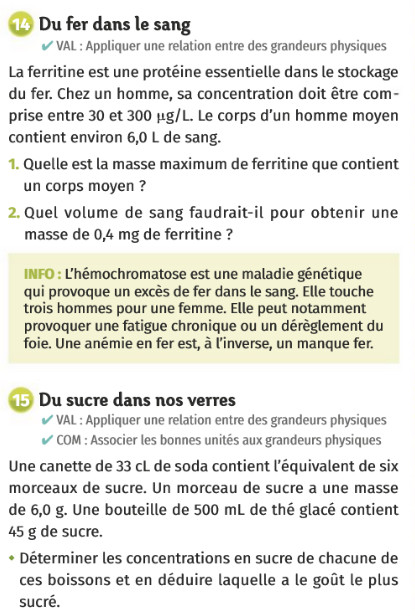
\includegraphics[scale=1.1]{Images/Ex_14.png}
\vspace{1cm}
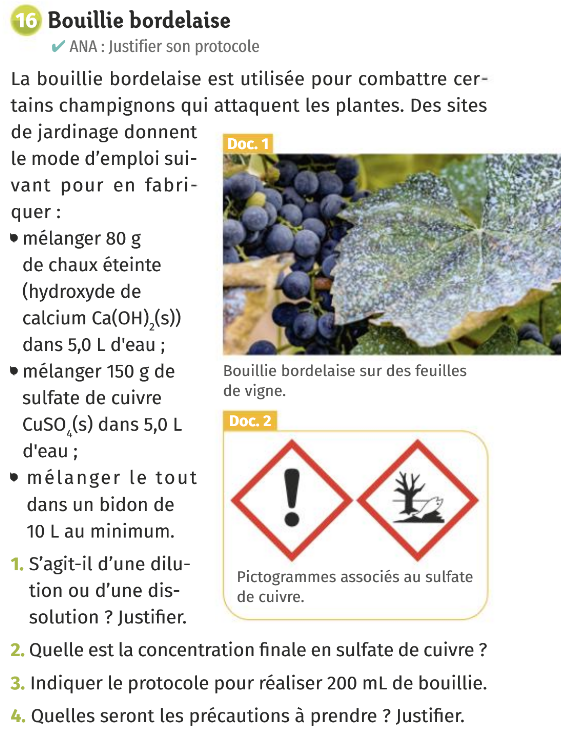
\includegraphics[scale=0.9]{Images/Ex_16.png}
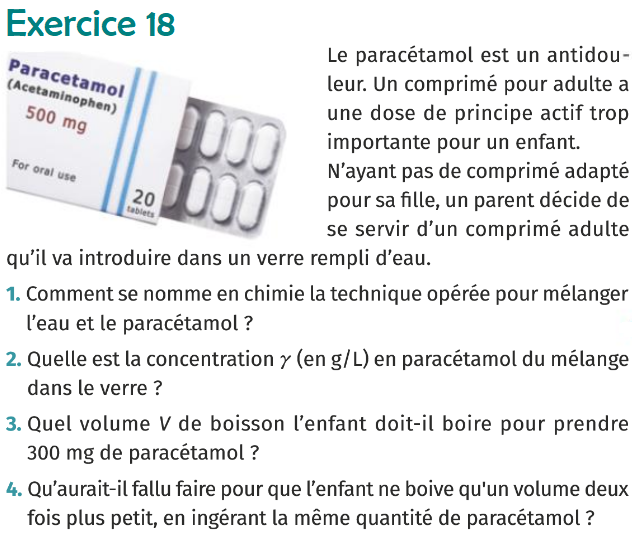
\includegraphics[scale=0.9]{Images/Exo_paracetamol.PNG}
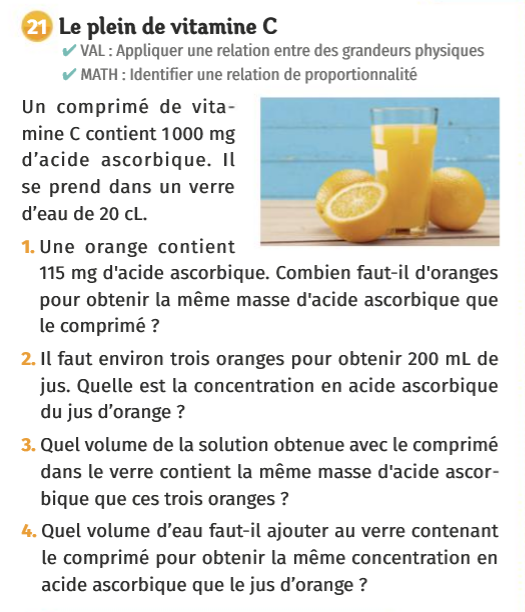
\includegraphics[scale=1.5]{Images/Ex_21.png}
\end{center}
\newpage
\begin{center}
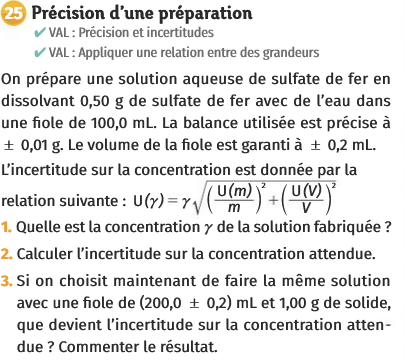
\includegraphics[scale=2]{Images/Ex_25.png}
\end{center}

\section{Pour aller plus loin}
\begin{center}
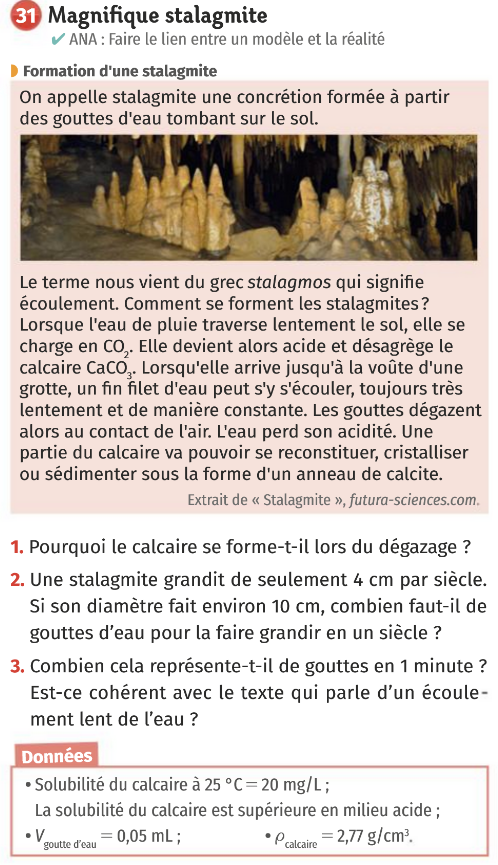
\includegraphics[scale=1.5]{Images/Ex_31.png}
\end{center}
\newpage
\begin{center}
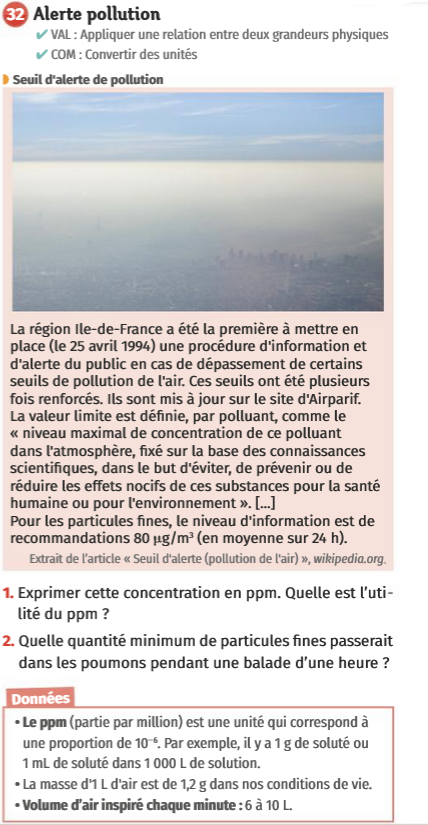
\includegraphics[scale=1.5]{Images/Ex_32.png}
\end{center}